\documentclass[a4paper, 10pt]{article}
\usepackage[top=3cm, bottom=2cm, left=1cm, right=1cm]{geometry}

\usepackage[utf8]{inputenc}
\usepackage[brazil]{babel}
\usepackage{indentfirst}
\usepackage{times}
\usepackage{lipsum}

\usepackage{amsmath, amsfonts, amssymb, mathtools, mismath}

\usepackage{indentfirst}
\usepackage{times}
\usepackage{titlesec}
\usepackage{cancel}

\usepackage{graphicx}

\usepackage{float}
\usepackage{tabularx, multirow, longtable, makecell}
\usepackage[thinlines]{easytable}

\usepackage{fancyvrb}
\usepackage{hyperref}

\usepackage{enumitem}

\newcommand{\limit}{\displaystyle\lim}
\newcommand{\integral}{\displaystyle\int}
\newcommand{\summation}{\sum\limits}
\newcommand\pd[2]{\displaystyle\frac{\partial #1}{\partial #2}}
\newcommand\der[3]{\displaystyle\frac{d^{#3} #1}{d #2^{#3}}}
\newcommand\blfootnote[1]{%
  \begingroup
  \renewcommand\thefootnote{}\footnote{#1}%
  \addtocounter{footnote}{-1}%
  \endgroup
}
\newcommand{\comment[1]}{\null}

\DeclareMathOperator{\sen}{sen}
\newcommand{\newspaceline}{\vspace{5pt}\\}
\pagestyle{empty}
\DeclareMathOperator{\rotg}{rot \,}
\usepackage{txfonts}
\usepackage{pdfpages}

\pagestyle{empty}

\begin{document}
    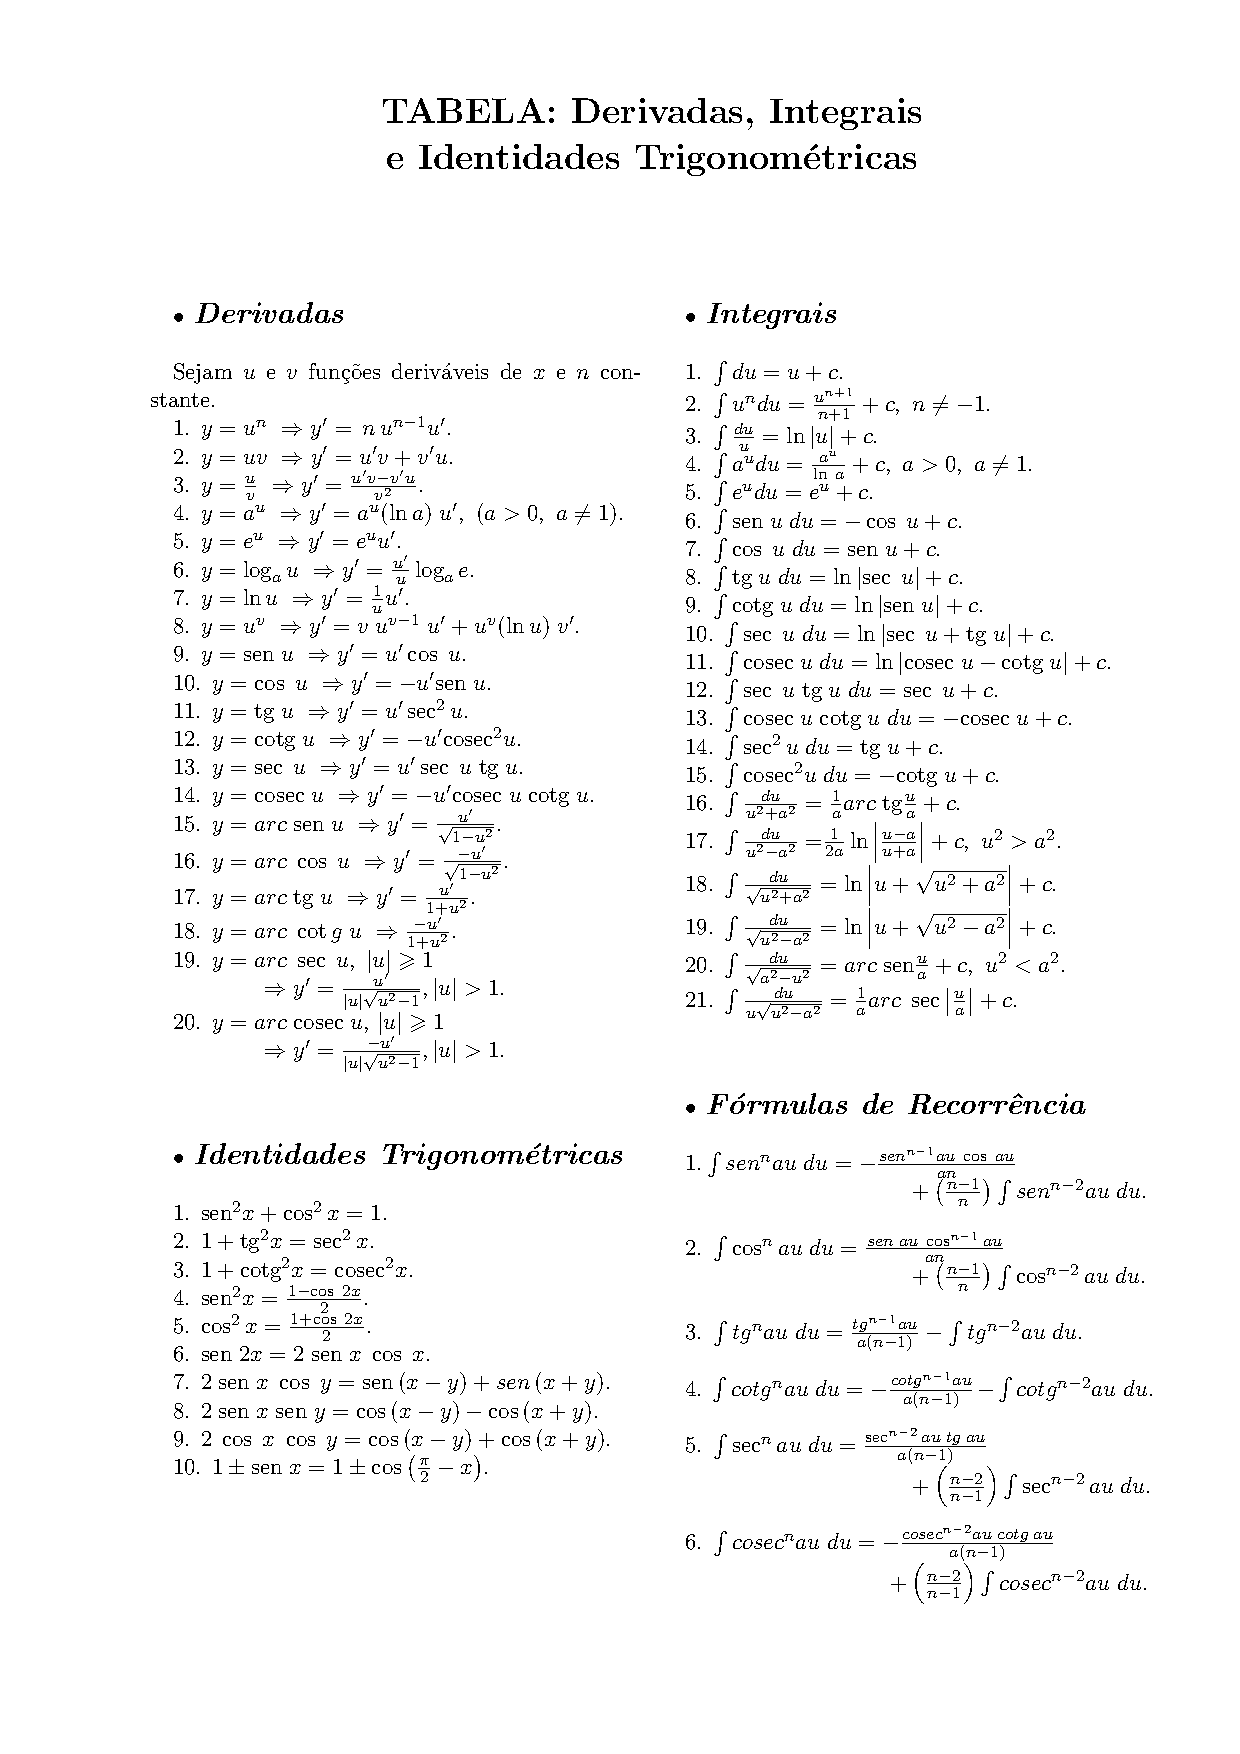
\includepdf[page=-]{alreadymadepdf/tab-integrais.pdf}
    \newpage
    		\begin{center}
		\begin{Huge}
			Resumo Cálculo Integral de Múltiplas Variáveis
		\end{Huge}\\		
		\hrulefill \vspace{12pt} \\	
		\begin{Large}
			Integrais Duplas e Triplas
		\end{Large}
	\end{center}
	
	\begin{large}
	Definição de Integral Dupla e Teorema de Fubini:
	\end{large}		
	\begin{gather*}
	\mathit{C}=[a,b]\times [c,d] = (x,y)\in\mathbb{R}^2: a\leq x\leq b, \,c \leq y\leq d	\\
	f:\textit{C}\to\mathbb{R} \text{ é contínua}\\
	I=\displaystyle\iint_{\mathit{C}}f(x,y)dA=\displaystyle\int_a^b\displaystyle\int_c^df(x,y)dxdy=
	\displaystyle\int_c^d\displaystyle\int_a^bf(x,y)dydx \text{\hspace{12pt}(Teorema de Fubini)}
	\end{gather*}
	
	\begin{large}
	Mudança de Variáveis:
	\end{large}
	\begin{gather*}
	f:\mathit{V}\to\mathbb{R}\\
	f\circ h: \mathit{U} \to \mathbb{R}\\
	I=\displaystyle\iint_{\mathit{V}}f(x,y)dxdy=\displaystyle\iint_{\mathit{U}}f(h(u,v))\;|\det Dh(u,v)|dudv \\
	\text{Onde $Dh$ é a matriz Jacobiana de $h$}
	\end{gather*}
	
	\begin{large}
	
	Coordenadas Polares:
	\end{large}
	\begin{gather*}
	r\in[0,+\infty), \,\theta\in[0,2\pi)\\
	h(r,\theta) = (x(r,\theta),y(r,\theta))=(r\cos\theta,r\sin\theta)\\
	\begin{cases}
	x=r\cos\theta \\
	y=r\sin\theta	
	\end{cases}\hspace{12pt}
	\begin{cases}
	r=\sqrt{x^2+y^2}\\
	\tan\theta=\dfrac{y}{x}	
	\end{cases}\\
	\det Dh(r,\theta)=\det\begin{bmatrix}
	x_r & x_\theta \\
	y_r & y_\theta
	\end{bmatrix}=\det\begin{bmatrix}
	\cos\theta & -r\sin\theta \\
	\sin\theta & r\cos\theta
	\end{bmatrix} = r
	\end{gather*}
	
	\begin{large}
	Definição de Integral Tripla e Teorema de Fubini:
	\end{large}		
	\begin{gather*}
	\mathit{C}=[a,b]\times [c,d] \times [r,s] = (x,y,z)\in\mathbb{R}^3: \begin{cases} a\leq x\leq b, \\ c \leq y\leq d, \\ r\leq z\leq s
	\end{cases}	\\
	f:\textit{C}\to\mathbb{R} \text{ é contínua}\\
	I=\displaystyle\iiint_{\mathit{C}}f(x,y,z)dV=\displaystyle\int_a^b\displaystyle\int_c^d
	\displaystyle\int_r^sf(x,y,z)dxdydz \\
	\text{Obs.: O Teorema de Fubini ainda pode ser utilizado.}
	\end{gather*}

	\begin{large}
	Coordenadas Esféricas:
	\end{large}
	\begin{gather*}
	\rho\in[0,+\infty), \,\theta\in[0,2\pi), \, \phi\in[0,\pi)\\
	r=\rho\sin\phi \rightarrow	
	\begin{cases}
	x=\rho\cos\theta\sin\theta \\
	y=\rho\sin\theta\cos\phi	
	\end{cases}\hspace{12pt}
	z=\rho\cos\phi \hspace{12pt} \rho=\sqrt{x^2+y^2+z^2}\\
	\det Dh(\rho,\theta\phi)= \rho^2\sin\phi
	\end{gather*}
	
	
	\begin{large}
	Coordenadas Cilíndricas:
	\end{large}
	\begin{gather*}
	r\in[0,+\infty), \,\theta\in[0,2\pi), 
	\, z\in(-\infty,+\infty)\\
	\begin{cases}
	x=r\cos\theta \\
	y=r\sin\theta	
	\end{cases}\hspace{12pt}
	r=\sqrt{x^2+y^2}\\
	\det Dh(r,\theta,z) = r
	\end{gather*}
	
	\newpage
	\begin{center}		
		\begin{Large}
			Curvas Parametrizadas(em $\mathbb{R}^2$ ou $\mathbb{R}^3$)
		\end{Large}
	\end{center}
	
	\begin{large}
	Integrais de Linha de Funções Reais:
	\end{large}
	\begin{gather*}
	\gamma:[a,b]\to\mathbb{R}^n \\
	\gamma(t)=(x_1(t),x_2(t),\ldots,x_n(t)), \hspace{12pt} \gamma'(t)=(x_1'(t),x_2'(t),\ldots,x_n'(t))\\
	f:\mathbb{R}^n\to\mathbb{R} \\
	f\circ \gamma (t) = f(\gamma (t))\\
	\displaystyle\int_\gamma f ds = \displaystyle\int_a^b f(\gamma (t))\|\gamma '(t)\| dt\\
	\|\gamma'(t)\|=\sqrt{\displaystyle\sum_{i=1}^n(x'_n(t))^2} = \sqrt{x_1'(t)^2+x_2'(t)^2+\ldots+x_n'(t)}
	\end{gather*}
	
	\begin{large}
	Integrais de Linha de Campos Vetoriais	
	\end{large}		
	\begin{gather*}
	U\subseteq\mathbb{R}^3 \text{aberto} \\
	X:U\to \mathbb{R}^3 \text{campo vetorial em $U$} \\
	(x,y)\in U \mapsto X(x,y)= (P(x,y,z),Q(x,y,z),R(x,y,z))\\
	\vspace{12pt}\\
	\gamma:[a,b] \to U \text{curva parametrizada}\\
	t \to (x(t),y(t),z(t)) \\
	\vspace{24pt}\\
	\displaystyle\int_\gamma Xd\vec{r}=\displaystyle\int_a^b\langle X(\gamma(t)), \gamma'(t) \rangle dt = \displaystyle\int_a^b(P\cdot x'(t) + Q\cdot y'(t) + R\cdot z'(t)) dt
	\end{gather*}
	
	\null\hspace{48pt}Obs.: $\langle v,w \rangle = \|v\|\|w\|\cos\theta$
	
	\begin{center}
	\fbox{
\begin{minipage}{\dimexpr\textwidth-50\fboxsep-2\fboxrule\relax}
Campos gradientes(ou conservativos):
\begin{gather*}
	U\subseteq\mathbb{R}^n \text{aberto, } f:U\to\mathbb{R}\\
\end{gather*}
Caso:
\begin{gather*}
	X(x_1,\ldots,x_n)=\nabla f(x_1,\ldots,x_n)=\left(\dfrac{\partial f}{\partial x_1}(x_1,\ldots,x_n),\ldots,\dfrac{\partial f}{\partial x_n}(x_1,\ldots,x_n)\right)\\
\end{gather*}
$X$ é conservativo.\\
Obs.:
\begin{gather*}
\forall v \in\mathbb{R}^n \setminus \{0\}:\\
\dfrac{\partial f}{\partial v}(x) = \langle\nabla f(x), v\rangle
\end{gather*}
\end{minipage}
}\end{center}

\null\hspace{48pt}Assim, se:
\begin{gather*}
X=\nabla f \, , \, \gamma:[a,b]\to\mathbb{R}^n/
\begin{cases}
\gamma(a)=A \\
\gamma(b)=B
\end{cases}\\
\displaystyle\int_\gamma \nabla fd\vec{r}=f(B)-f(A)
\end{gather*}
 
\begin{center}
\fbox{
\begin{minipage}{\dimexpr\textwidth-50\fboxsep-2\fboxrule\relax}
Em resumo, as seguintes afirmações são equivalentes:
\begin{enumerate}
\item $X$ é um campo gradiente: $\exists f:U \to \mathbb{R}/X=\nabla f$;
\item A integral de $X$ ao longo de caminhos fechados depende apenas do ponto inicial e final;
\item $\displaystyle\oint_\gamma X d\vec{r} = 0$ para qualquer curva fechada $\gamma$
\end{enumerate}
\end{minipage}
}\end{center}

\begin{center}
\fbox{
\begin{minipage}{\dimexpr\textwidth-50\fboxsep-2\fboxrule\relax}

Fórmula de Green:
\begin{gather*}
U \subset \mathbb{R}^3\text{ aberto limitado, com fronteira $\partial U$} \\
\partial U \text{ é uma curva fechada orientada positivamente}\\
X=(P,Q)\text{ campo de vetores de classe $C^1$ em U e $\partial U$}\\
\displaystyle\oint_{\partial U} X d\vec{r} = -\displaystyle\iint_U\underbrace{\left(\dfrac{\partial P}{\partial y} - \dfrac{\partial Q}{\partial x}\right)}_{\rotg X} dA
\end{gather*}
\end{minipage}
}\end{center}

	\begin{large}
	Dois operadores diferenciais:
	\end{large}
	\begin{center}
	\begin{align*}
	\text{Divergência:}&
	\begin{cases}
	\divg X:U\to\mathbb{R}\hspace{6pt} / \\
	\divg X(x,y) = \dfrac{\partial P}{\partial x}(x,y) + \dfrac{\partial Q}{\partial y}(x,y)
	\end{cases} \\
	\text{Rotacional:}&
	\begin{cases}
	\rotg X:U\to\mathbb{R}\hspace{6pt} / \\
	\rotg X = \dfrac{\partial Q}{\partial x}(x,y) - \dfrac{\partial P}{\partial y}(x,y)
	\end{cases}
	\end{align*}
	\end{center}
	
\begin{large}
Integrais de Linha de Campos Vetoriais em $\mathbb{R}^2$
\end{large}\\
\begin{gather*}
U\subseteq\mathbb{R}^2 \text{	aberto} \\
X = (P,Q) \text{	campo vetorial em $U$} \\
(x,y)\in U \mapsto X(x,y) = (P(x,y),Q(x,y))
\end{gather*}	

\begin{center}
\fbox{
\begin{minipage}{\dimexpr\textwidth-50\fboxsep-2\fboxrule\relax}
Fórmula de Green:
\begin{gather*}
U \subset \mathbb{R}^2\text{ aberto limitado, com fronteira $\partial U$} \\
\partial U \text{ é uma união finita de curvas fechadas orientadas positivamentes}\\
X=(P,Q)\text{ campo de vetores de classe $C^1$ em U e $\partial U$}\\
\displaystyle\oint_{\partial U} X d\vec{r} = -\displaystyle\iint_U\underbrace{\left(\dfrac{\partial P}{\partial y} - \dfrac{\partial Q}{\partial x}\right)}_{\rotg X} dA
\end{gather*}
\end{minipage}
}\end{center}

\null\hspace{48pt}Obs.: Se $X$ é um campo gradiente, então $\displaystyle\oint_\gamma X d\vec{r}=0$ para qualquer curva fechada $\gamma$\\	


\begin{center}		
		\hrulefill \vspace{12pt} \\	
		\begin{Large}
			Superfícies em $\mathbb{R}^3$
		\end{Large}
	\end{center}

\begin{large}
	Tipos de superfícies:
\end{large}
\begin{enumerate}
\item Gráfico de funções reais de duas variáveis:
\begin{gather*}
U \subseteq \mathbb{R}^2 \text{, } f:U\to\mathbb{R} \\
\{ (x,y,z) \in \mathbb{R}^3: (x,y) \in U \text{; } z \in f(x,y) \}
\end{gather*}
\item Superfícies de nível:
\begin{gather*}
V \subseteq \mathbb{R}^3 \text{, } f:V\to\mathbb{R}\text{, } c \in \mathbb{R} \\
\{ (x,y,z) \in V: f(x,y,z)=c \}
\end{gather*}
\item Superfícies de revolução
\end{enumerate}

\begin{large}
	Superfícies parametrizadas: $U \subseteq \mathbb{R}^n$ aberto
\end{large}
\begin{gather*}
\Phi :U\to\mathbb{R}^3 \text{ de classe } C^1 \text{, injetora e tal que } D\Phi(u,v) \text{ que também é injetora} \\ \Phi(u,v)=(x(u,v),y(u,v),z(u,v))\\
\Im(\Phi) = S \text{ que é uma suérfície}\\
D\Phi(u,v)=\left( \dfrac{\partial \Phi}{\partial u}, \dfrac{\partial \Phi}{\partial v}, \hat{i}+\hat{j}+\hat{k}\right) = \begin{pmatrix}
\hat{i} & \hat{j} & \hat{k} \\
x_u & y_u & z_u \\
y_v & y_v & z_v
\end{pmatrix}
\end{gather*}
\null\hspace{48pt}$C$ plano tangente à superfície parametrizada por $\Phi$ é gerado pelos vetores $\dfrac{\partial \Phi}{\partial u}$ e $\dfrac{\partial \Phi}{\partial v}$\\
\null\hspace{48pt}Um vetor normal é dado então pelo produto vetorial de $\dfrac{\partial \Phi}{\partial u}$ e $\dfrac{\partial \Phi}{\partial v}$:

\begin{gather*}
\text{
\begin{minipage}{68pt}
Vetor unitário \\ e ortogonal\\ à superfície
\end{minipage}}\hspace{10pt}\longrightarrow \hspace{10pt}
\zeta (u,v) = \dfrac{\dfrac{\partial \Phi}{\partial u} \times \dfrac{\partial \Phi}{\partial v}}{\left\lVert \dfrac{\partial \Phi}{\partial u} \times \dfrac{\partial \Phi}{\partial v}\right\rVert}
\end{gather*}

\null\hspace{48pt}A área da superfície é dada por:
\begin{gather*}
A(s)=\displaystyle\iint_U \left\lVert \dfrac{\partial \Phi}{\partial u} \times \dfrac{\partial \Phi}{\partial v}\right\rVert \underbrace{dA}_{dudv}
\end{gather*}

\begin{large}
Integrais em superfícies em $\mathbb{R}^3$
\end{large}
\begin{gather*}
U \subseteq \mathbb{R}^2 \\
\Phi(u,v) :U\to \mathbb{R}^3 \\
f(x,y):\mathbb{R}^2\to \mathbb{R}\\
\displaystyle\iint_S fdS = \displaystyle\iint_U f(\Phi (u,v))\left\lVert \dfrac{\partial \Phi}{\partial u}(u,v) \times \dfrac{\partial \Phi}{\partial v}(u,v)\right\rVert \underbrace{dA}_{dudv}
\end{gather*}

\begin{large}
Integrais de campos de vetores em $\underbrace{\text{superfícies orientáveis}}_{\text{(admite um campo normal unitário)}}$
\end{large}

\begin{gather*}\text{
Seja $S$ superfície orientável com campo normal $\zeta$ e $X$ um campo de vetores em $\mathbb{R}^3$} \\
\text{O fluxo de $X$ através de $S$ é dado por}: \\
\displaystyle\iint_S\langle X,\zeta \rangle dS = \displaystyle\iint_U \langle X(\Phi(u,v), \pm \left\lVert \dfrac{\partial \Phi}{\partial u}(u,v) \times \dfrac{\partial \Phi}{\partial v}(u,v)\right\rVert \rangle \underbrace{dA}_{dudv}
\end{gather*}

\begin{large}
Teorema de Gauss
\end{large}\vspace{12pt}\\
\null\hspace{48pt} \begin{minipage}{\dimexpr\textwidth-30\fboxsep-2\fboxrule\relax}
Seja $\Omega \subset \mathbb{R}^3$ aberto limitado cuja fronteira $\partial\Omega$ é uma superfície parametrizada orientável orientada com a normal exterior a $\Omega$. Seja $X$ um campo de vetores de classe $C^1$ em $\Omega \cup \partial\Omega$:
\end{minipage}

\begin{gather*}
\displaystyle\oiint_{\partial\Omega} \langle X, \zeta \rangle dS = \displaystyle\iiint_{\Omega} \divg X dV
\end{gather*}

\null\hspace{48pt}Obs.: $\begin{cases} U \subseteq \mathbb{R}^3 \text{ aberto} \\ X=(P,Q,R) \text{ campo em } U\\
f:U\to\mathbb{R}\\ \divg X = \dfrac{\partial P}{\partial x} +\dfrac{\partial Q}{\partial y}+\dfrac{\partial R}{\partial z}\end{cases}$

\begin{center}
\fbox{
\begin{minipage}{\dimexpr\textwidth-50\fboxsep-2\fboxrule\relax}
Observações
\begin{enumerate}
\item Se $X$ é um campo gradiente, então: $\rotg X \equiv 0$
\item Se $X$ é um campo gradiente qualquer, então: $\divg\rotg X =0$
\end{enumerate}
\end{minipage}
}\end{center}

\begin{large}
Teorema de Stokes
\end{large}\vspace{12pt}\\
\null\hspace{48pt} \begin{minipage}{\dimexpr\textwidth-30\fboxsep-2\fboxrule\relax}
Seja $S \subset \mathbb{R}^3$ superfície orientável, orientada pelo vetor normal $\zeta$, cuja fronteira $\partial S$ é uma curva de classe $C^1$ com a orientação induzida. \\
E $X$ campo de vetores de classe $C^1$ em um aberto contendo $S \cup \partial S$.
\end{minipage}
\begin{gather*}
\displaystyle\oint_{\partial S} X d\vec{r} = \displaystyle\iint_S \langle \rotg X, \zeta \rangle dS
\end{gather*}

    \newpage
    	\begin{center}
		\begin{Huge}
			Métodos de Resolução de EDOs
		\end{Huge}\\		
		\hrulefill \vspace{12pt} \\	
		\begin{Large}
			EDOs de primeira ordem
		\end{Large}
	\end{center}				
	\begin{table}[H]
		\begin{center}
		\begin{TAB}(r,0.1cm,1cm)[5pt]{|c|c|c|}{|c|c|}
 			Variáveis separáveis & $y'=f(x)g(y)$ & $\displaystyle\int \dfrac{1}{g(y)}dy=\displaystyle\int f(x)dx$ \\
 			Fator Integrante & $y'+P(x)y=Q(x)$ & $I(x)y(x)=\displaystyle\int I(x)Q(x) dx$, onde $I=\exp{\left(\displaystyle\int P(x)dx\right)}$
		\end{TAB}
		\end{center}
	\end{table}
	\begin{center}		
		\hrulefill \vspace{12pt} \\	
		\begin{Large}
			EDOs exatas
		\end{Large}
	\end{center}
		\begin{table}[H]
		\begin{center}
		\begin{TAB}(r,0.1cm,1cm)[5pt]{|c|c|c|}{|ccc|cc|}
 			Caso geral & $M(x,y)dx+N(x,y)dy = 0$ & caso $\dfrac{\partial N}{\partial x} = \dfrac{\partial M}{\partial y}$ \\ 			& & temos $\dfrac{\partial G}{\partial x} = M(x,y)$ e $\dfrac{\partial G}{\partial y} = N(x,y)$,\\
 			& &  e $G(x,y)=K$ é solução. \\
 			Das não exatas às exatas & $IM(x,y)dx + IN(x,y)dy = 0$ & onde $I=I(x)$ ou $I=(y)$ e \\
 			& & $\dfrac{\partial (IM)}{\partial y} = \dfrac{\partial (IN)}{\partial x}$
		\end{TAB}
		\end{center}
	\end{table}
	\begin{center}		
		\hrulefill \vspace{12pt} \\	
		\begin{Large}
			EDOs homogêneas
		\end{Large}
	\end{center}
		\begin{table}[H]
		\begin{center}
		\begin{TAB}(r,0.1cm,0.25cm)[2pt]{|c|c|c|}{|cc|c|}
 			Mudança de variável & $y'=F\left(\dfrac{y}{x}\right)$ & $y=u \cdot x$\\
 			& &  $y'=u'x+u \rightarrow u'x=F(u)-u$ \\
 			Como saber se é homogênea? & $\begin{cases} x \rightarrow kt \\ y \rightarrow kt \end{cases}$ & $y'=f(x,y)=f(kx,ky)$
		\end{TAB}
		\end{center}
	\end{table}
	\newpage
	\begin{center}		
		\hrulefill \vspace{12pt} \\	
		\begin{Large}
			EDOs de ordem $n=2$
		\end{Large}
	\end{center}
	\hspace{2cm}Obs.:\begin{minipage}[t]{\textwidth}
		Soma de soluções também é solução, portanto $y_1$ e $y_2$ são soluções individuais. \\
		$W(f,g)$ é o Wronskiano de $f$ e $g$.
		\end{minipage}		 
		\begin{table}[H]
		\begin{center}
		\begin{TAB}(r,0.01cm,0.02cm)[0.5pt]{|c|c|c|}{|c|c|c|c|c|c|}
 			\makecell{Coeficientes constantes\\(Caso homogêneo)} & $a_0y+a_1y'+a_2y''=0$ & \makecell{Equação característica: $a_0+a_1\alpha+a_2\alpha^2=0$\\$y=y_1+y_2$\\
 			Se $\begin{cases} \Delta > 0 \rightarrow y(x)=C_1e^{\lambda_1x}+C_2e^{\lambda_2x} \\ 
 			\Delta = 0 \rightarrow y(x)=C_1xe^{\lambda x} + C_2e^{\lambda x} \\ \Delta<0 \rightarrow y(x)=C_1e^{ax}\cos(bx) + C_2e^{ax}\sin(bx) \end{cases}$\\
 			Onde $\lambda$ é raiz real e $a\pm bi$ são raizes complexas} \\
 			Caso não homogêneo & $a_0y+a_1y'+a_2y''=g(x)$ &
 			\makecell{$y=y_h+y_p$\\Onde $y_h$ é a solução da homogênea e\\ $y_p$ é uma solução particular}\\
 			\makecell{Método de variação de parâmetros \\ (Encontrar soluções particulares)} & $y_p=C_1y_1+C_2y_2$ & \makecell{$C_1 = \displaystyle\int\dfrac{-y_2 \cdot g(x)}{a_2 \cdot W(y_1,y_2)}dx$ \\$C_2 = \displaystyle\int\dfrac{y_1\cdot g(x)}{a_2\cdot W(y_1,y_2)}dx$} \\ EDO de Cauchy-Euler & $ax^2y''+bxy'+cy=0$ & \makecell{Eq. inicial: $am(m-1)+bm+c=0$\\Se $\begin{cases} \Delta > 0 \rightarrow y(x)=C_1x^{m_1}+C_2x^{m_2} \\ 
 			\Delta = 0 \rightarrow y(x)=C_1x^m+C_2\ln(x)\cdot x^m \\ \Delta<0 \rightarrow y(x)=x^{\alpha}(C_1\cos(\beta\ln x)+C_2\sin(\beta\ln x))\end{cases}$ \\ Onde $m$ é raiz real e $\alpha\pm\beta i$ é raiz complexa} \\
 			EDO de Bessel & \makecell{$x^2y''+xy'+(\lambda^2x^2-p^2)=0$\\Com $p\in\mathbb{R}$ constante} & \makecell{Se$\begin{cases}p\in\mathbb{Z} \rightarrow y(x)=C_1J_p(x)+Y_p(x)\\
 			p\not\in\mathbb{Z} \rightarrow y(x)=C_1J_p(x)+C_2J_{-p}(x) \end{cases}$\\ Onde $J_p$ é a função de Bessel de 1ª espécie de ordem $p$\\e $Y_p$ é a função de Bessel de 2ª espécie de ordem $p$\\Nota: $\lim_{x\to0^+}Y_p(x)=-\infty$}\\
 			EDO de Legendre & \makecell{$p\in\mathbb{R}$ constante\\ com $y(x):(-1,1)\to\mathbb{R}$\\$(1-x^2)y''+2xy'+p(p+1)y=0$} & \makecell{Se $p=n\in\mathbb{N}$\\$y(x)=C_1P_n(x)+C_2Q(x)$\\Onde $P_n$ é a função de Legendre de 1ª espécie de ordem $n$\\e $Q_p$ é a função de Legendre de 2ª espécie de ordem $n$\\Nota: $\lim_{x\to1^-}Q_n(x)=+\infty$}
		\end{TAB}
		\end{center}
	\end{table}	
	
	\hspace{2cm}Lembretes: \begin{minipage}[t]{\textwidth}
$e^{i\theta}=\cos(\theta)+i\sin(\theta)$ \\ $\sin(\theta)=\dfrac{e^{i\theta}-e^{-i\theta}}{2i}=\dfrac{\sinh(i\theta)}{i}$ \; e \;$\cos(\theta)=\dfrac{e^{i\theta}+e^{-i\theta}}{2}=\cosh(i\theta)$ \\ A redução de ordem é um algoritmo capaz de reduzir a ordem de EDOs, porém não será detalhado.
		\end{minipage}	
	
	\newpage
	\begin{center}		
	\hrulefill \vspace{12pt} \\	
	\begin{Large}
		Outros métodos de resolução
	\end{Large}
	\end{center}

	\begin{table}[H]
		\begin{center}
		\begin{TAB}(r,0.1cm,0.25cm)[2pt]{|c|c|c|}{|c|c|}			
 			Séries de potências & $\displaystyle\sum_{k=0}^if_i(x)y^{(i)}=g(x)$ & $y(x)=\displaystyle\sum_{n=0}^\infty C_nx^n$ 
\\ Transformada de Laplace & $\displaystyle\sum_{k=0}^if_i(x)y^{(i)}=g(x)$ com PVI & Aplicar $\mathcal{L} \rightarrow$ Resolver Eq. Algébrica $\rightarrow$ Aplicar $\mathcal{L}^{-1}$
		\end{TAB}
		\end{center}
	\end{table}

    \newpage
    		\begin{center}
		\begin{Huge}
			Critérios de convergência para séries
		\end{Huge}\\		
		\hrulefill
	\end{center}			

	\textbf{Critério da Divergência} \\
Seja $\summation_n a_n$ uma série. Se $\limit_{n \to \infty} a_n \ne 0$, então $\summation_n a_n$ é divergente. \newspaceline

\textbf{Critério da Integral}\\
Seja $\summation_n a_n$ uma série e seja $m$ um natural tal que $a_n\ge0$ para todo $n\ge m$. Suponha uma $f(x)$ que no intervalo $\left[m,+\infty\right)$ satisfaz as seguintes condições:
\begin{itemize}[noitemsep, nolistsep]
	\item É contínua;
	\item descrescente;
	\item não negativa;
	\item e tal que $f(n)=a_n$ para todo natural $n\ge m$.
\end{itemize}
Temos que a série $\summation_n a_n$ é convergente se e somente se a integral imprópria $\integral_m^{+\infty}f(x)dx$ é convergente. \newspaceline

\textbf{Critério da comparação direta}\\
Sejam $\summation_n a_n$ e $\summation_n b_n$ duas séries e seja $m$ um número natural tal $b_n\ge a_n \ge 0$ para todo $n\ge m$, temos:
\begin{enumerate}[noitemsep, nolistsep]
	\item  Se $\summation_n b_n$ é convergente, então a série $\summation_n a_n$ é convergente.
	\item Se $\summation_n a_n$ é divergente, então a série $\summation_n b_n$ é divergente.
\end{enumerate}
\vspace{5pt}

\textbf{Critério da comparação no limite}\\
Sejam $\summation_n a_n$ e $\summation_n b_n$ duas séries e seja $m$ um número natural tal $a_n\ge 0$ e $ b_n \ge 0$ para todo $n\ge m$, suponha o seguinte limite:
$$L = \limit_{n\to\infty}\dfrac{a_n}{b_n}$$
exista, então.
\begin{enumerate}[noitemsep, nolistsep]
	\item Se $L\ne 0$ então $\summation_n a_n$ converge se e somente se $\summation_n b_n$ converge.
	\item Se $L=0$ e $\summation_n b_n$ converge, então $\summation_n a_n$ converge.
\end{enumerate}

\textbf{Critério da série alternada}\\
Seja $\summation_n a_n$ uma série alternada com $\left| a_n \right| = b_n$, a série é convergente se satisfaz os seguintes critérios:
\begin{enumerate}[noitemsep, nolistsep]
	\item $b_{n+1} \le b_n$ para todo $n\ge m$;
	\item e $\limit_{n \to \infty} b_n = 0$
\end{enumerate}
para algum $m \in \mathbb{N}$.
\newspaceline

\textbf{Convergência absoluta}\\
Se a série $\summation_{n=1}^{\infty} \left| a_n \right|$ é convergente, então $\summation_{n=1}^{\infty} a_n$ é convergente. \\
Obs.: a volta não é garantida.
\newspaceline

\textbf{Critério da razão}\\
Seja $\summation_{n=1}^{\infty} a_n$ uma série com todos os termos não nulos e seja $r=\limit_{n \to\infty} \dfrac{\left| a_{n+1} \right|}{\left| a_n \right|}$. Então:
\begin{enumerate}[noitemsep, nolistsep]
	\item Se $r<1$, a série $\summation_{n=1}^{\infty} a_n$ converge absolutamente.
	\item Se $r>1$ (incluindo $r\to+\infty$), a série $\summation_{n=1}^\infty a_n$ diverge.
\end{enumerate}
\vspace{5pt}

\textbf{Critério da raiz}\\
Sejam $\summation_{n=1}^\infty a_n$ uma série e $r=\limit_{n \to\infty}\sqrt[n]{\left| a_n \right|}$. Então:
\begin{enumerate}[noitemsep, nolistsep]
	\item Se $r<1$, a série $\summation_{n=1}^\infty a_n$ converge absolutamente.
	\item Se $r>1$ (incluindo $r\to+\infty$), a série $\summation_{n=1}^\infty a_n$ diverge.
\end{enumerate}


    \newpage
    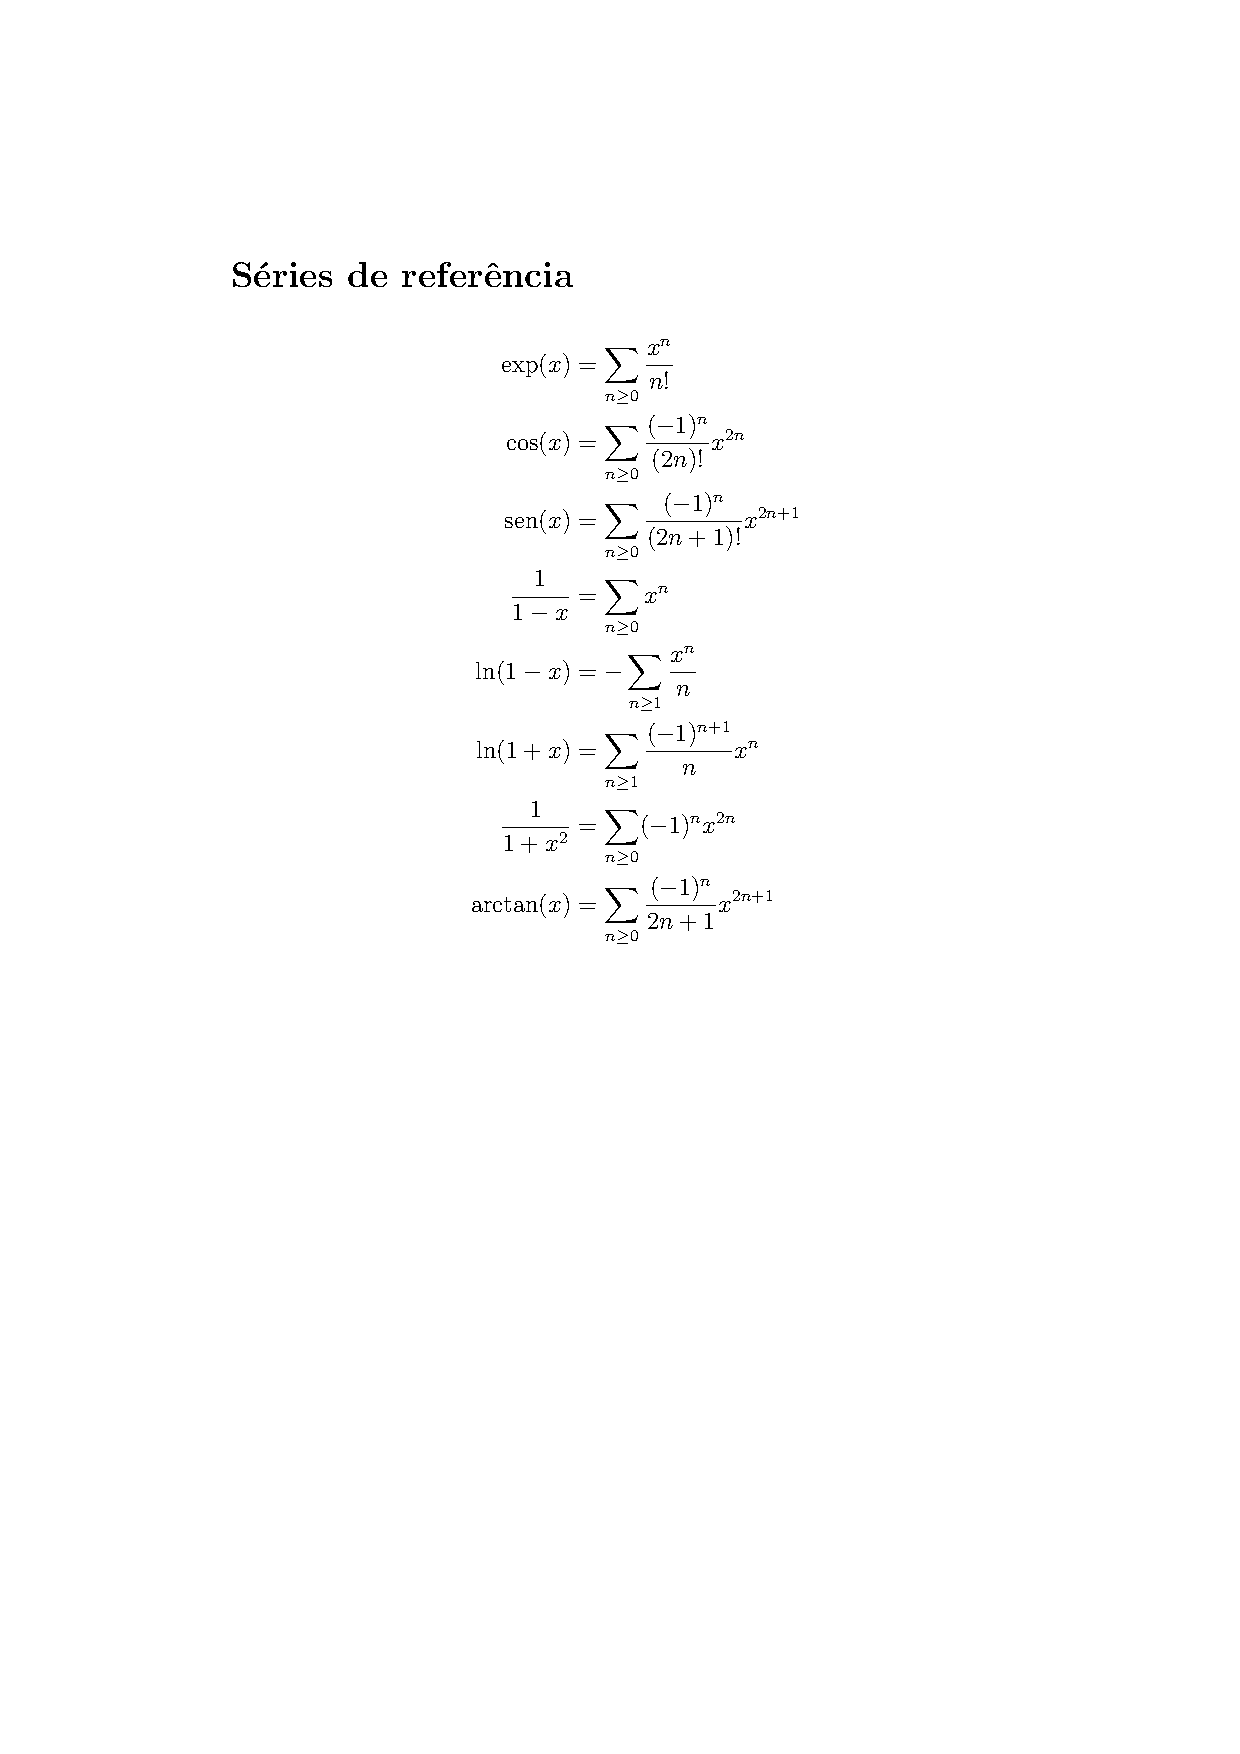
\includepdf[page=-]{alreadymadepdf/Tabela-series.pdf}
    \newpage
    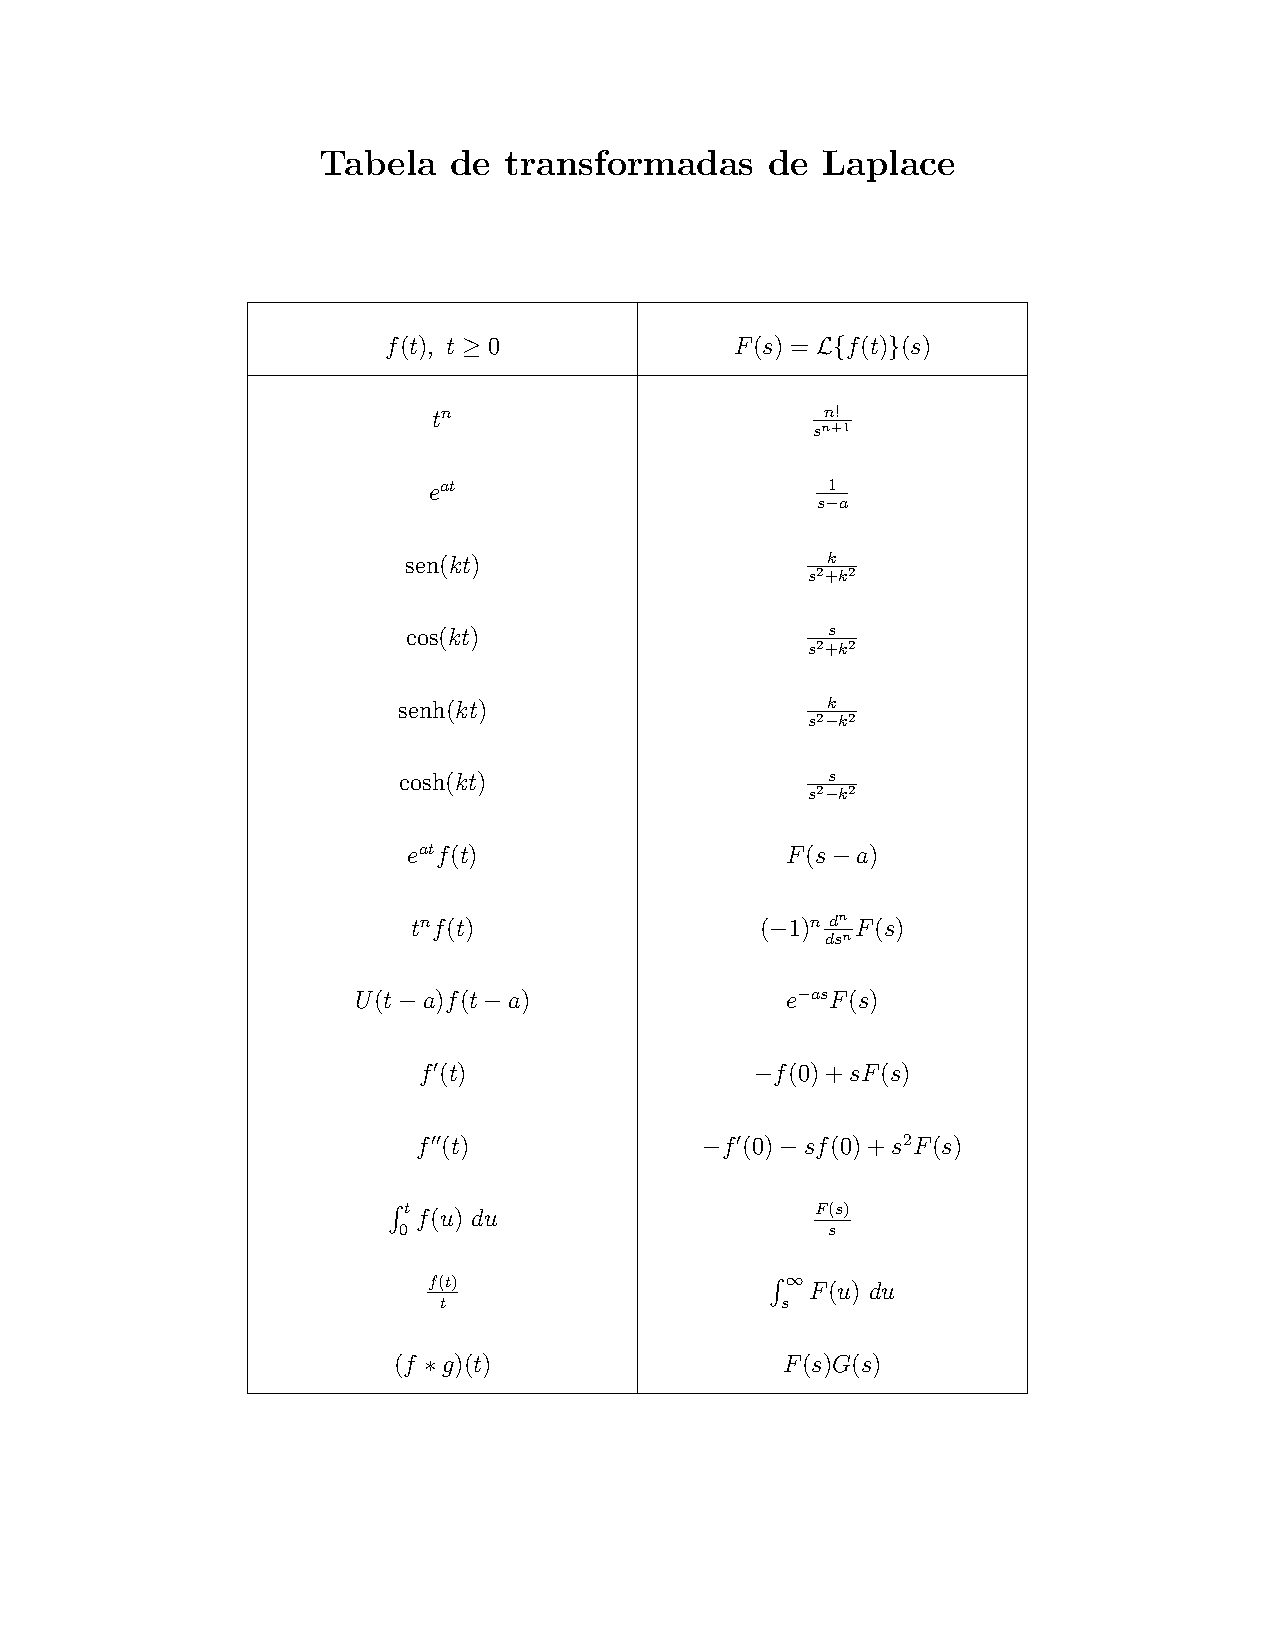
\includepdf[page=-]{alreadymadepdf/Tabela-Laplace.pdf}
\end{document}

